\subsection{Bonita}
\begin{quotation}
Le BPM est la discipline de la gestion des processus (plutôt que des tâches) en tant que moyen d'améliorer les résultats de performance de l'entreprise et l'agilité opérationnelle. \cite{gartnerdic}
\end{quotation}

Bonita est une plate-forme basé sur BPM qui sert à construire des applications, personnalisées, en prenant l'avantage plein du BPM pour s'adapter aux changements en temps réel.

La plate-forme a deux parties. Voir Figure \ref{fig:bonita_archi}:
\begin{itemize}
  \item Bonita Studio
  \item Bonita Plate-forme (Bonita Engine)
\end{itemize}

\subsubsection{Bonita Studio}
Bonita le Studio est un environnement graphique pour créer des processus, des applications, des modèles de données et des vues d'utilisateurs. Il contient trois outils de design(conception) majeurs:

\begin{itemize}
  \item Le tableau blanc, pour dessiner un organigramme de processus et définir les transitions.
  \item Le menu de Développement, pour étendre les capacités du Studio et crée les modèles de données.
  \item Le Concepteur UI, qui est utilisé pour créer des pages d'application et des formulaires de processus
\end{itemize}

Le Studio contient une Plate-forme Bonita (Tomcat, UI Designer, Bonita Portal, Bonita Engine et une base de données H2), approprié pour tester une application

\subsubsection{Bonita Engine}
C'est le runtime processeur au cœur de Bonita. Il exécute des processus, en traitant des actions liées aux tâches, comme l'accès de base de données. Le Moteur est composé d'un certain nombre de services et API. Les services sont services BPM ou des services génériques.

\begin{figure}[!ht]
\centering
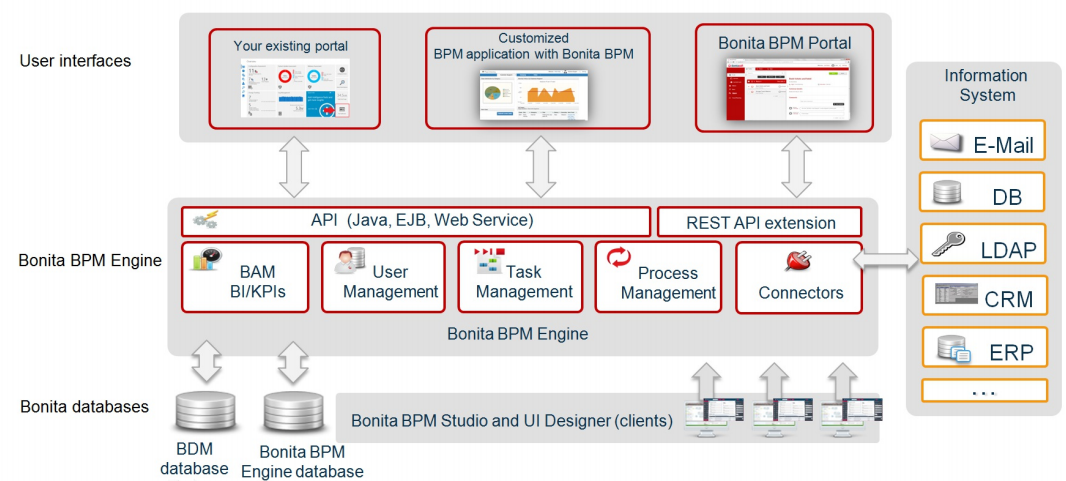
\includegraphics[width=\textwidth,keepaspectratio]{bonita_archi.png}
\caption{Bonita Architecture}
\label{fig:bonita_archi}
\end{figure}
